\chapter{Acoustics and Digital Signal Processing}
\label{ch:speech analysis}
In the past decade, digital computers have significantly helped \textit{signal processing} to quantify a finite number of bits. The flexibility inherited from digital elements allowed the usage of a vast number of techniques in which had not been possible to implement in the past. Nowadays, digital signal processor have been used to perform multiple operations, such as \textit{filtering}, \textit{spectrum estimation} and many others algorithms \cite{orfanidis1995introduction}.


\section{Speech signals}
\label{sec:speech_signals}
The \textbf{speech} is the human way of communication. The protocol used in communication is based on a syntactic combination of different words taken from a very large vocabulary. Each word in the vocabulary is composed by a small set of vowels and consonants that combined with a phonetic unit forms a spoken word. \\
\noindent When a word is pronounced\footnote{\ref{ch:english_language} explains in details how phonemes are pronounced}, a sounds is produced causing the air particles to be excited at a certain vibration rate. The source of our voice is due to the vibration of the vocal cords. The resultant signal is \textit{non-stationary} but it can be divided in segments since each phoneme has a common acoustic properties. In \ref{fig:ex_sound_wave} it is possible to notice how the pronounced words have a different shape as well as when the intensity of the voice is higher/lower during the pronunciation.

\begin{figure}[!ht]
	\centering
	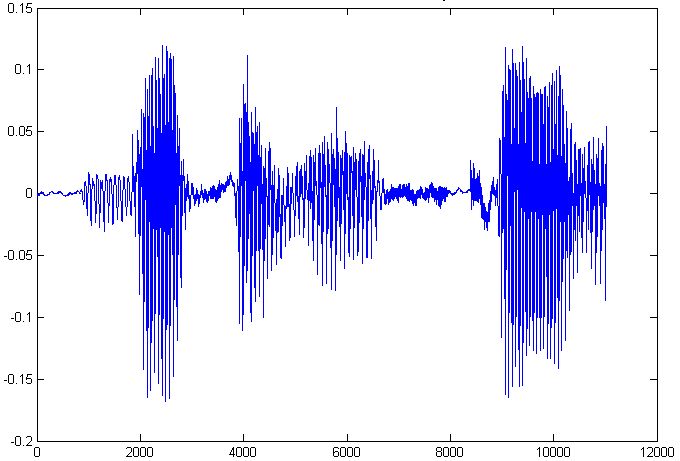
\includegraphics[scale=0.4]{Figures/ex_speech.png}
	\caption{Example of a speech sound. In this case, the sentence \textbf{This is a story} has been pronounced \cite{ex_speech_image}}
	\label{fig:ex_sound_wave}
\end{figure}

\noindent The simplest form of sound is the \textit{sinusoid} and it is the easiest waveform to describe because it corresponds to a \textbf{pure tone}. A pure tone consist in a waveform that consists only on one frequency. Other examples are the \textit{cosine} or \textit{sine} waves.

\subsection{Properties of Sinusoids}
\label{sub:prop_of_sinusoids}
A sinusoid is a simple waveform represented by a up and down movement. There are three important measures that must be taken into consideration when defining the shape of the sinusoid: \textit{amplitude}, \textit{frequency} and \textit{phase}.

\subsubsection{Amplitude}
The amplitude, from a sound point of view, corresponds to the \textit{loudness} whereas in the soundwave it corresponds to the amount of \textbf{energy}. In general, to measure the amplitude, we use the unit called \textbf{deciBels} (dB) in which it is measured using a logarithmic scale relative to a standard sound \cite{prop_of_sinusoids}.

\subsubsection{Frequency}
Frequency is the number of cycles per unit of time\footnote{In general, a unit of time is considered a single second}.To define cycle, we can think of an oscillation that starts from the middle line, goes to the maximum point, down to the minimum and get back to the middle point. The unit of measure of the frequency is calculated in \textbf{Hertz} (Hz). Also, if we calculate the time taken for one cycle, we estimate the so called \textbf{period}. \\
\noindent Frequency plays a fundamental role with the \textit{pitch}. In fact, changing the number of oscillations but keeping the same waveform, we are able to increase or decrease the level of the pitch.

\subsubsection{Phase}
The \textbf{phase} measures the starting point position of the waveform. If the sinusoids start at the very minimum of the wave, the value of the phase is $\pi$ radians whereas starting from the top of the wave it will have a phase of \textit{zero}. When two sounds do not have the same phase, it is possible to perceive the difference in the time scale since one of the two is delayed compared to the other. When comparing two signals, there is the need to obtain a \textit{"phase-neutral"}, that means the comparison is made taking only Amplitude and Frequency into account. This method is called \textbf{autocorrelation} of the signals.

\subsection{Spectrograms}
\label{sec:spectrograms}
A \textbf{spectrogram} is the visual representation of an acoustic signal \cite{spectrogram_def}. Basically, a Fourier Transformation is applied to the sound, in such a way to obtain the set of waveforms extracted form the original signal and separate their frequencies and amplitudes. The result is typically depicted in a graph with degrees of amplitude with a \textit{light-dark} representation. Since amplitude represents the \textit{energy}, having a darker shade means that the energy is more intense in a certain range of frequencies - lighter when there is low energy. In \ref{fig:nasal_spectrogram} there is an example of the spectrogram. \\
\noindent The visual feedback of the spectrogram is highly dependent from the \textbf{window size} of the Fourier Analysis. In fact, different sizes affect the levels of frequencies and time resolution. \\
\noindent If the window size is \textit{short}, the adjacent \textbf{harmonics} are distorted but the time resolution is better \cite{spectrogram_def}. An harmonic is an integer multiple of the fundamental frequency or component frequencies. This is helpful when we are looking for the \textit{formant structure} because the striations created by the spectrogram highlights the individual pitch periods. \\
\noindent On the other hand, a \textit{wider} window size, helps to locate the harmonics because the band of the spectrogram are narrower.


\section{Fourier Analysis}
\label{sec:fourier_analysis}
\textbf{Fourier Analysis} is the process of decomposing a periodic waveform into a set of sinusoids having different amplitudes, phases and frequencies. Yet, if we add those waveforms again, we will obtain the original signal. The analysis has been involved in many scientific applications and the reason is due to the following transform properties:

\begin{itemize}
	\item Linear transformation - the relationship between two modules is kept
	\item Exponential function are eigenfunctions of differentiation \cite{evans1997partial}
	\item Invertible - derived from the linear relationship
\end{itemize}

\noindent In signal processing, the Fourier analysis is used to isolate singular components of a complex waveform. A set of techniques consist in using \textbf{Fourier Transformation} on a signal in such a way to be able to manipulate the data in the easiest way possible but at the same time we have to be capable of inverting the transformation \cite{rabiner1975theory}. In the next subsections we describe the fundamental steps for manipulating a signal.

\subsubsection{Sampling}
\label{ssubs:sampling}

\textit{Sampling} is the process where a continuous signal is periodically measured every \textbf{T} seconds \cite{orfanidis1995introduction}. \\
\noindent Consider a sound signal that varies in time as a continuous function $s(t)$. For every $T$ seconds, we need to measure the value of the function. This frame of time is called the \textit{sampling interval} \cite{weik2012communications}. To calculate the sequence a sampled function is given as follow: $s(nT), \forall$ integer values of $n$. Thus, the \textit{sampling rate} is the average number of samples obtained in a range of $T = 1sec$ \cite{sampling_wiki}. An example of sampling is shown in \ref{fig:sampling_ex}.

\begin{figure}[!ht]
	\centering
	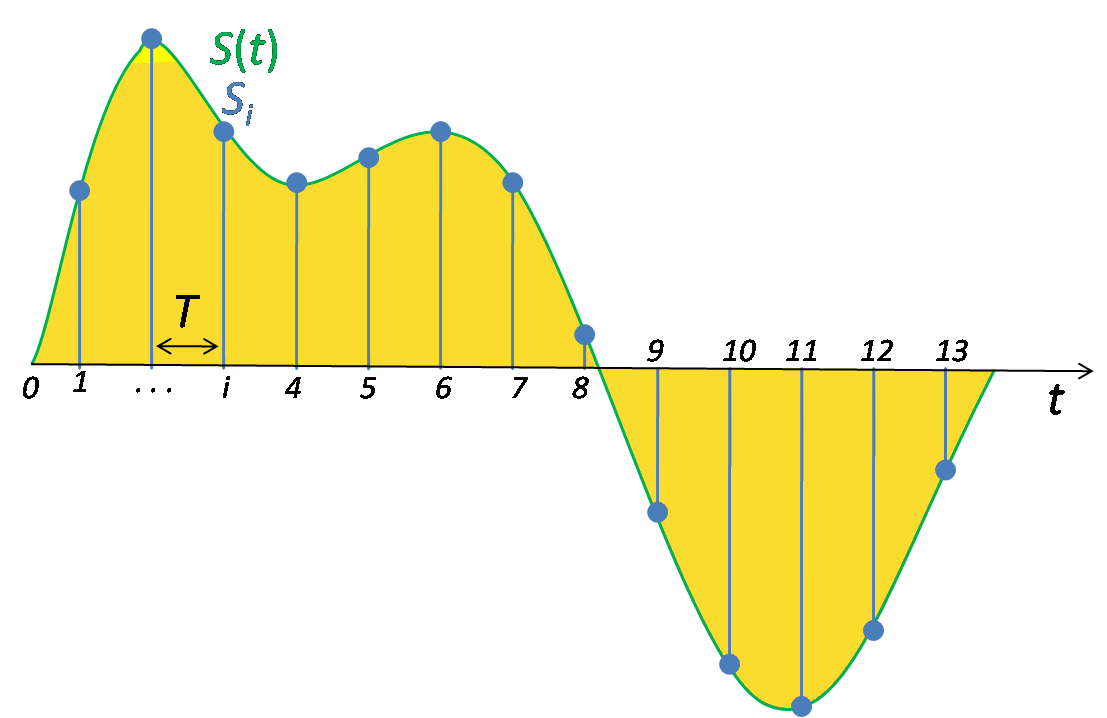
\includegraphics[scale=0.2]{Figures/sampling_example.png}
	\caption{Example of signal sampling. The green line represents the continuous signal whereas the samples are represented by the blue lines \cite{sampling_wiki}}
	\label{fig:sampling_ex}
\end{figure}

\noindent As we mentioned above, using the Fourier Analysis we need to be able to reconstruct the original signal from the transformed one. To be able to, the \textbf{Nyquist-Shannon} theorem states that the sampling rate has to be larger as twice as the maximum frequency of the signal, in order to rebuild the original signal \cite{sampling_illinois}.\\
\noindent The \textit{Nyquist sampling rate} is defined by the following equation:

\begin{equation}
f_{s} > f_{Nyquist} = 2f_{max}
\end{equation}


\subsubsection{Quantization}
\label{subs:quantization}
To finalize the transformation from a continuous signal to a discrete one, we need to \textit{quantized} the signal in such a way to obtain a finite set of values. Unlike sampling, in which permits to reconstruct the original signal, quantization is an irreversible operation that introduce a loss of information. \\
\noindent Consider $x$ be the sampled signal and $x_{q}$ the quantized one where $x_{q}$ can be expressed as the signal $x$ plus the error $e_{q}$. From here we have:

\begin{equation}
x_{q} = x + e{q} \Leftrightarrow e_{q} = x - x_{q}
\end{equation}

Given the equation above, we can restrict the range of error to $-q/2 ... +q/2$ because we will not make a larger error than the half of the quantization step. From a mathematical point of view, the error-signal is a random signal with an uniform probability distribution between the range of $−q/2 and +q/2$, giving the following \cite{quantization_math}:

\begin{equation}
p(e) = \begin{Bmatrix}
			\frac{1}{q} & for \frac{-q}{2} \leq  e < \frac{q}{2}\\
			0 			& otherwise
		\end{Bmatrix}
\end{equation}

Given this reason, the quantization error also called quantization noise.

\subsubsection{Windowing Signals}
\label{ssubs:windowing_signals}
Speech sound is a \textbf{non-stationary} signal where its properties (amplitude, frequency and pitch) rapidly change over time \cite{windowing_fi}. Due to the quick changes of those properties, it makes it hard to use \textit{autocorrelation} or \textit{Discrete Fourier Transformation}. In \ref{ch:english_language} we highlighted the fact that phonemes have some invariant properties for a small period of time. Having said that, it is possible to apply methods that will take \textit{short windows} (pieces of signal) and process them. This window is also called \textbf{frame}. Typically, the shape of this window is \textit{rectangular} because one of the most used methods are the \textit{Hanning} and \textit{Hamming} in which the window covers the whole amplitude spectrum between a range. In \ref{fig:windowing_ex} there is an example on how the Hamming window is taken from a signal. The rectangle called \textit{Time Record}, is the frame that is extracted and processed by the windowing function.

\begin{figure}[!ht]
	\centering
	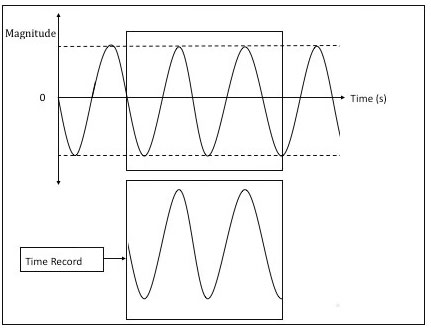
\includegraphics[scale=0.5]{Figures/windowing.png}
	\caption{Hamming window example on a sinusoid signal}
	\label{fig:windowing_ex}
\end{figure}


\subsubsection{Hann Function}
\label{ssubs:hann_function}
This is one of the most used windowing method in signal processing. The function is discrete and it is defined by \ref{eq:discrete_window_function}. The method is a linear combination of the \textit{rectangular function} defined by \ref{eq:rectangular_function}. Starting from the \textit{Euler's formula}, it is possible to inject the rectangular equation as in \ref{eq:euler_formula}. From here, given the properties of the \textit{Fourier Transformation}, the spectrum of the window function is defined as in \ref{eq:spectrum_ft}. Combining the spectrum with \ref{eq:rectangular_function} we obtain \ref{eq:final_hann} in which the signal modulation factor \textit{disappears} when the windows are moved around time $0$.

\begin{subequations}
\label{eq:hann_function_equations}
\begin{align}
w(n) &= 0.5 \left(1 - \cos \left ( \frac{2 \pi n}{N-1} \right) \right) \label{eq:discrete_window_function} \\
w_r &= \mathbf{1}_{[0,N-1]} \label{eq:rectangular_function} \\
w(n) &= \frac{1}{2} \,w_r(n) -\frac{1}{4} e^{\mathrm{i}2\pi \frac{n}{N-1}} w_r(n) - \frac{1}{4}e^{-\mathrm{i}2\pi \frac{n}{N-1}} w_r(n) \label{eq:euler_formula} \\
\hat{w} (\omega) &= \frac{1}{2} \hat{w}_r (\omega) - \frac{1}{4} \hat{w}_r \left(\omega + \frac{2\pi}{N-1}\right) - \frac{1}{4} \hat{w}_r \left(\omega - \frac{2\pi}{N-1}\right) \label{eq:spectrum_ft} \\
\hat{w}_r (\omega) &= e^{-\mathrm{i} \omega \frac{N-1}{2}} \frac{\sin(N\omega/2)}{\sin(\omega/2)} \label{eq:final_hann}
\end{align}
\end{subequations}

\noindent The reason why this windowing method is one of the most diffuse is due to the \textit{low aliasing}

\subsubsection{Zero Crossing Rate}
\label{ssubs:Zero Crossing Rate}
Zero crossing is the point of the function where the sign changes from a positive value to a negative one or vice versa. The method of counting the zero crossings is widely used in speech recognition for estimating the \textit{fundamental} frequency of the signal. The zero-crossing rate is the rate of this positive-negative changes. Formally, it is defined as follow:

\begin{equation}
ZCR = \frac{1}{T-1} \sum_{t=1}^{T-1} \begin{Bmatrix}
										1  & s_t s_{t-1} < 0 \\
										0 & otherwise
									 \end{Bmatrix}
\end{equation}

\noindent where $s$ is the signal of length $T$.

\subsubsection{The Discrete Fourier Transform}
\label{ssubs:discrete_fourier_transform}
Before jumping into the definition of the Discrete Fourier Transformation (DFT), we need to introduce the Fourier Transformation (FT) from the mathematical point of view. The FT of a continuous-signal $x(t)$ is defined by the following equation:

\begin{equation}
X(\omega) = \int_{-\infty}^\infty x(t)e^{-j\omega t} dt, \qquad \omega\in(-\infty,\infty)
\end{equation}

\noindent The discrete operation allows us to transform the equation above from an infinite space in a finite sum as follows:
\begin{equation}
X(\omega_k ) = \sum_{n=0}^{N-1}x(t_n)e^{-j\omega_k t_n}, \qquad k=0,1,2,\ldots,N-1
\end{equation}

where $x(t_n)$ is the \textit{amplitude} of the signal at time $t_n$ (sampling time). $T$ is the sampling period in which the transformation is applied. $X(\omega_k )$ is the \textit{spectrum} of the complex value $x$ at frequency $\omega_k$. $\Omega$ is the sampling interval defined by the \textit{Nyquist-Shannon} theorem whereas $N$ is the number of samples. \\

\noindent The motivation behind the DFT is that we want to move the signal from the \textit{Time or space domain} to the \textit{Frequency domain}. This allows us to analyze the spectrum in a simpler way. \ref{fig:dft} shows the transformation.

\begin{figure}[!ht]
	\centering
	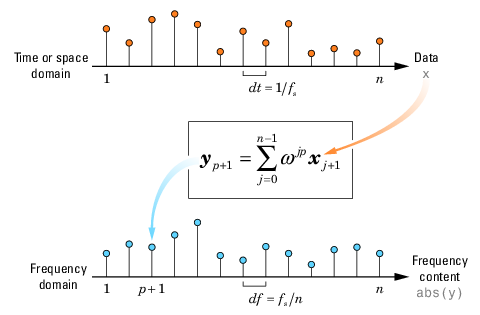
\includegraphics[scale=0.7]{Figures/dft.png}
	\caption{DFT transformation \cite{dft_matlab}}
	\label{fig:dft}
\end{figure}
